\documentclass[a4paper,11pt,twocolumn]{article}
\usepackage{mathtools}
\usepackage{esvect}

\usepackage{titling}

\setlength{\droptitle}{-10em}

\setlength{\intextsep}{6pt plus 1.0pt minus 2.0pt}

\title{Applications of PCA and Image Compression (Lab 1)}

\date{November 21, 2017}

\author{
  Samuil Dichev, mbaxtsd2\\
  \texttt{The University of Manchester}\\
}

\begin{document}

\maketitle

\section{Applications of PCA}
The iris dataset becomes easier to analyse in lower dimensions without the redundancy. Figure \ref{fig:fig1} shows clearly linearly separable data, as does Figure \ref{fig:fig2}, which also shows tighter clustering for parts of the data. Not much can be analysed without the labels, but with them one could draw better conclusions from seeing the data represented in the these subspaces.
\\Figure \ref{fig:fig3} on the other hand, doesn't reveal much information about the data. There is no clear separation and there is little to no clustering to speak of.
From observing the 3 figures, we can clearly see the principal components' variance reduces from first to last, as it should.

\begin{figure}[!h]
  \centering
  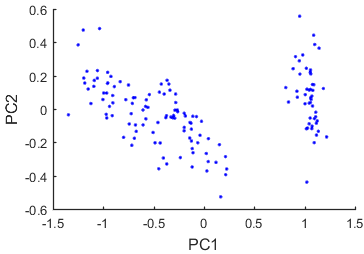
\includegraphics[width=\linewidth]{figures/PC1-PC2.png}
  \caption{Results in subscape $PC_1$-$PC_2$.}
  \label{fig:fig1}
\end{figure}

\begin{figure}[!h]
  \centering
  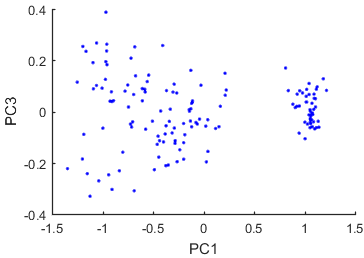
\includegraphics[width=\linewidth]{figures/PC1-PC3.png}
  \caption{Results in subscape $PC_1$-$PC_3$.}
  \label{fig:fig2}
\end{figure}

\begin{figure}[!h]
  \centering
  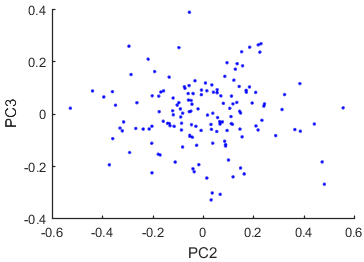
\includegraphics[width=\linewidth]{figures/PC2-PC3.png}
  \caption{Results in subscape $PC_2$-$PC_3$.}
  \label{fig:fig3}
\end{figure}

\section{Image Compression}
For the image compression of the digits, I used PCA with SVD because the data has more dimensions (features) than examples. Since our examples are images, each pixel of the images is a feature. At a width by height of 28 by 28, that's 784 pixels or 784 features. The images (examples), however, were only 300 in the train dataset.
\\\\
For the implementation of this compression system, I designed a function to represent the training data as a matrix of size 784x300, where each column is each 28x28 image represented as a column vector instead of a matrix. This was then passed though the pca2 function, which returned the PCs. The number of PCs to use was chosen based on Proportion of Variance $PoV >= 90\%$, calculated via:
$$PoV = \frac{\sum_{i=1}^{k} \lambda_{i}}{\sum_{i=1}^{d} \lambda_{i}}$$

This condition is first satisfied at 47 principal components with $PoV = 90.05\%$. By comparison, at $k = 46$ we only get a PoV of 89.77\%, so $k = 47$ is the first value at which we achieve a satisfactory $PoV >= 90\%$ as shown in Figure \ref{fig:fig4}.

\begin{figure}[!h]
  \centering
  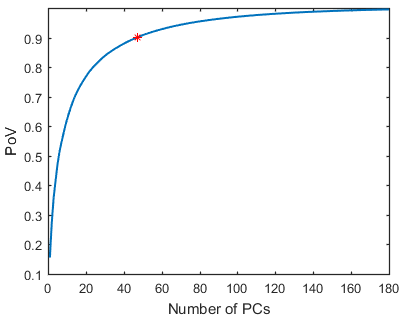
\includegraphics[width=\linewidth]{figures/PoV.png}
  \caption{PoV for each k. Marker at $k = 47$.}
  \label{fig:fig4}
\end{figure}

At 47 principal components, we also observe a good size compression on disk. After using matlab's save function to save each dataset on disk separately, I established that the default uncompressed test dataset is of size 4985 bytes, while the compressed version of the test dataset is only 3837 bytes, which is a size compression of roughly 23.03\%.
\\\\Each datapoint is compressed via $z = U^{T}_{M}(x - \vv{x})$ and is then reconstructed via $x' = \vv{x} + U_{M}z$
\\\\On Figure \ref{fig:fig5} we can see the original test dataset images, before any compression and on Figure \ref{fig:fig6} we can see the same images after reconstruction using 47 PCs.
\\\\On Figure \ref{fig:fig7} we see the reconstructed images. The left column contains the images compressed and reconstructed using 1 to 25 PCs and the right column shows the images made with PCs between 26 and 50.\\\\ 

\begin{figure}[!h]
  \centering
  
\includegraphics[width=\linewidth]{img/original.png}
  \caption{Original uncompressed test images.}
  \label{fig:fig5}
\end{figure}

\begin{figure}[!h]
  \centering
  
\includegraphics[width=\linewidth]{img/47pcs.png}
  \caption{Reconstructed images using 47 PCs.}
  \label{fig:fig6}
\end{figure}

\begin{figure}[!h]
  \centering
  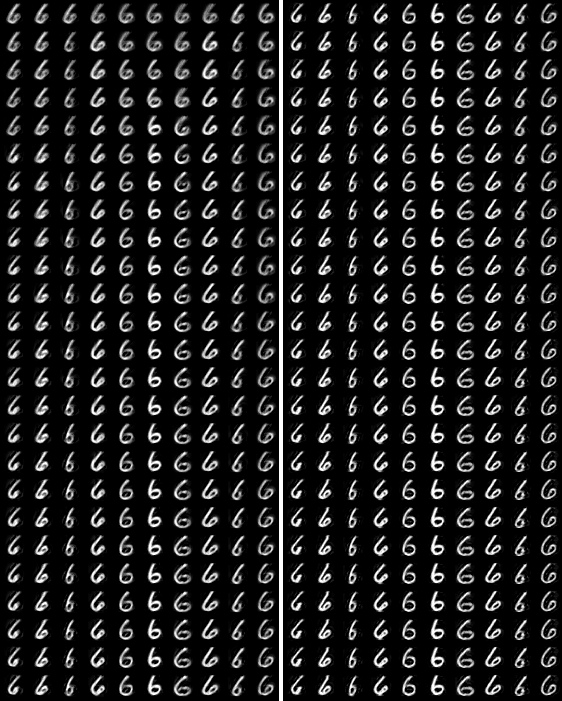
\includegraphics[width=\linewidth]{img/1to50.png}
  \caption{Reconstructed images in order of number of PCs used from 1 to 50.}
  \label{fig:fig7}
\end{figure}

\end{document}